\documentclass[aps,pra,reprint,superscriptaddress,nofootinbib]{revtex4-2}
\usepackage{amsmath,amssymb,bm}
\usepackage{graphicx}
\usepackage{booktabs}
\usepackage{hyperref}
\usepackage{tikz}
\usetikzlibrary{arrows.meta,positioning,fit,calc}
\usepackage{pgfplots}
\usepgfplotslibrary{groupplots}
\pgfplotsset{compat=1.18}
\newcommand{\GQ}{G_{\mathrm Q}}
\newcommand{\GA}{G_{\mathrm A}}
\newcommand{\Tr}{\operatorname{Tr}}

\begin{document}
\title{Accessible Quantum Natural Gradient: Optimizing in the Geometry Seen by the Readout}
\author{Marwan Ait Haddou}
\affiliation{Independent Researcher, Morocco}
\date{\today}

\begin{abstract}
Quantum natural gradient (QNG) preconditions variational optimization with the full quantum Fisher geometry of a parameterized state, although a learning model generally interacts with that state only through a fixed measurement and a restricted family of retained observables. We introduce the accessible quantum natural gradient (AQNG), an optimization rule obtained by replacing the full state-space metric by the pullback of measurement--readout-accessible tangent geometry. The construction is the algorithmic consequence of the spectral accessibility framework, which separates quantum tangent sensitivity from the fraction exposed by measurement and readout. We compare AQNG with full QNG on four binary classification benchmarks, four six-qubit circuit families, and 20 paired stochastic seeds per dataset--architecture cell, for 640 terminal method rows. For the three nonconserving architectures, AQNG improves mean test accuracy in nine of twelve settings. The strongest behavior occurs for the SU(2)-Haar architecture, where the accessible metric retains only about 26--27\% of the full-QFIM trace while AQNG improves mean accuracy on all four datasets. Holm-corrected paired loss tests remain significant for Iris/SU(2)-Haar, Wine/SU(2)-Haar, and Digits/SU(2)-CNOT. In the implemented simulator stack AQNG reduces wall-clock time by factors of roughly 11--39, although this timing comparison is backend-specific and is not an intrinsic complexity claim. A number-conserving $U(1)$ control remains at fixed chance-like accuracy under both AQNG and full QNG despite high update-direction alignment, showing that fidelity to the full natural-gradient direction is not sufficient when the architecture/readout geometry is not useful for the supervised task. These results distinguish full quantum geometry, measurement-accessible geometry, and task-useful optimization geometry.
\end{abstract}
\maketitle

\section{Introduction}
The quantum Fisher information matrix (QFIM) equips a parameterized quantum state with a local information geometry and underlies the quantum natural-gradient update \cite{Braunstein1994,Stokes2020}. This geometry is measurement independent: it quantifies local distinguishability available in the state before a particular experimental interface is fixed. Variational quantum learning, by contrast, is normally driven by a restricted classical record, for example Pauli expectation values, low-order correlators, or marginals. Consequently, the optimizer need not have operational access to every direction represented by the full QFIM.

Our earlier work made this separation explicit. Under joint state--tangent isotropy, a fixed basis followed by a rank-$r$ diagonal readout retains a dimension-controlled fraction of the visible score information \cite{AitHaddouRank}. The subsequent spectral theory removed the isotropy requirement and represented measurement/readout accessibility by a positive contraction $T_{\mathcal M,\mathcal A}$ acting on normalized quantum tangent space \cite{AitHaddouSpectral}. If $C_Q$ denotes the orientation covariance of normalized quantum tangents, the ensemble-averaged accessible fraction is
\begin{equation}
 \mathbb E\!\left[\frac{I_{\mathcal M,\mathcal A}}{F_Q}\right]=\Tr(T_{\mathcal M,\mathcal A}C_Q).
 \label{eq:master}
\end{equation}
The isotropic readout-rank law is recovered as a special case when $C_Q$ is proportional to the identity on the relevant tangent space.

Equation~\eqref{eq:master} suggests an optimization question distinct from estimating the full QFIM: if the learning interface exposes only a contracted tangent geometry, should the optimizer precondition the loss gradient with directions that the interface does not retain? Here we answer this question constructively by introducing the \emph{accessible quantum natural gradient} (AQNG). AQNG is not defined as a numerical approximation whose sole objective is to reproduce the full QNG matrix. Instead, it uses the metric induced by retained measurement/readout tangent features. An accessible metric may carry only a modest fraction of QFIM trace and nevertheless generate a useful optimization direction.

We test this principle on four binary classification tasks and four circuit architectures. AQNG and full QNG share the same initial circuit, data split, stochastic seed, loss gradient, and training budget within each comparison. The results reveal three regimes. SU(2)-Haar provides a positive case in which a low-trace accessible metric is sufficient and frequently superior in generalization. SU(2)-CNOT and RyRz-CZ show architecture- and dataset-dependent behavior rather than universal dominance. Finally, a number-conserving $U(1)$ circuit provides a negative control: AQNG and full-QNG update directions are highly aligned, yet both remain at fixed chance-like classification accuracy. Natural-gradient fidelity therefore cannot compensate for a task-misaligned model/readout interface.

\section{Accessible tangent geometry}
\subsection{From quantum sensitivity to accessible sensitivity}
Let $|\psi_{\bm\theta}\rangle$ be a differentiable pure state and $X_v$ the horizontal tangent generated by parameter-space direction $v$. Its directional QFI is $F_Q(v)=4\langle X_v,X_v\rangle$. A measurement $\mathcal M$ maps the quantum tangent to a classical score tangent, and a retained readout space $\mathcal A$ projects that score onto directions represented by the chosen observables. The spectral accessibility framework packages the two contractions into
\begin{equation}
 T_{\mathcal M,\mathcal A}=A_{\mathcal M}^{\dagger}P_{\mathcal A}A_{\mathcal M},\qquad 0\preceq T_{\mathcal M,\mathcal A}\preceq I,
\end{equation}
so that for a normalized quantum tangent $u$,
\begin{equation}
 \frac{I_{\mathcal M,\mathcal A}(u)}{F_Q(u)}=\langle u,T_{\mathcal M,\mathcal A}u\rangle.
\end{equation}
For a differentiable classical head built from retained expectations, the effective first-order observable remains in the retained span. The first-order loss response is therefore bounded by accessible information, motivating the use of the same tangent span to define the optimizer metric.

\subsection{Accessible pullback metric}
The full QNG metric is the pure-state QFIM pullback
\begin{equation}
 (\GQ)_{ij}=4\,\mathrm{Re}\!\left[\langle\partial_i\psi|\partial_j\psi\rangle-\langle\partial_i\psi|\psi\rangle\langle\psi|\partial_j\psi\rangle\right].
\end{equation}
Let $\Phi_{\mathcal M,\mathcal A}$ map a horizontal quantum tangent to its retained covariance-normalized readout score. We define
\begin{equation}
 (\GA)_{ij}=\left\langle\Phi_{\mathcal M,\mathcal A}(\partial_i\psi),\Phi_{\mathcal M,\mathcal A}(\partial_j\psi)\right\rangle.
 \label{eq:GA}
\end{equation}
Thus $\GA$ is the parameter-space pullback of accessible tangent geometry and ideally satisfies $0\preceq\GA\preceq\GQ$. The damped updates compared here are
\begin{align}
 \Delta\bm\theta_{\rm QNG}&=-\eta(\GQ+\lambda I)^{-1}\nabla L,\\
 \Delta\bm\theta_{\rm AQNG}&=-\eta(\GA+\lambda I)^{-1}\nabla L.
\end{align}
The goal is not $\GA\simeq\GQ$ in matrix norm. The operational question is whether the accessible preconditioner preserves or improves directions that matter to the task.

\subsection{Nested readout probes}
The implementation diagnoses three nested diagonal readout spaces: a minimal probe $A_1$, the full local-$Z$ span, and the joint span of diagonal Pauli strings through weight two, denoted $\mathcal A_{\le2}$. The main AQNG metric uses the $\le2$ accessible geometry. The expected nesting is
\begin{equation}
 G_{A_1}\preceq G_{\rm local}\preceq G_{\le2}\preceq\GQ.
\end{equation}
We record metric rank, trace retention $\Tr(G_{\mathcal A})/\Tr(\GQ)$, and cosine between the resulting preconditioned direction and the full-QNG direction.

\section{Experimental design}
\subsection{Benchmarks and circuits}
We use four binary classification benchmarks: Iris, Breast Cancer, Wine, and Digits. Each experiment uses a fixed train/test split per dataset while the stochastic circuit/training seed is varied. The benchmark configuration uses six qubits, 80 samples, three variational layers, and 20 training steps. Four circuit families are compared: \texttt{ryrz\_cz}, \texttt{su2\_cnot}, \texttt{su2\_haar}, and the number-conserving \texttt{u1\_rzxy}. The $U(1)$ family is retained as a symmetry-constrained control because previous accessibility calculations show that its tangent orientation differs strongly from generic isotropic behavior \cite{AitHaddouRank,AitHaddouSpectral}.

\subsection{Optimization protocol}
AQNG and full QNG use learning rate $\eta=0.03$ and damping $\lambda=10^{-3}$. The loss minibatch contains eight examples, the metric minibatch contains four, and the metric is refreshed every two optimization steps. Each dataset--architecture cell contains 20 paired seeds, yielding $4\times4\times20=320$ paired comparisons and 640 terminal method rows. The initial loss gradient is shared within each pair; the recorded initial-gradient cosine is numerically unity.

\subsection{Statistics and timing}
For each cell we report mean test loss and accuracy over 20 seeds. Paired loss differences are $\Delta L=L_{\rm AQNG}-L_{\rm QNG}$, so negative values favor AQNG. Two-sided Wilcoxon signed-rank tests are corrected across the 16 cells by Holm's procedure. Wall-clock measurements refer only to the implemented simulator stack. The AQNG and full-QNG metric paths use different simulator backends in the present implementation while the loss path is shared; timing is therefore an implementation result, not an intrinsic quantum-resource claim.

\section{Results}
\subsection{Predictive performance}
Excluding the symmetry-constrained $U(1)$ control, AQNG improves mean test accuracy in nine of twelve dataset--architecture cells (Table~\ref{tab:acc}). The result is not universal: RyRz-CZ favors full QNG on Iris and Digits, and SU(2)-CNOT is essentially tied on Breast Cancer. This heterogeneity supports an architecture-dependent accessible-geometry picture rather than a claim of universal optimizer dominance.

\begin{table*}
\caption{Mean test accuracy over 20 paired seeds. Values are percentages. $\Delta$ is AQNG minus full QNG in percentage points.}
\label{tab:acc}
\begin{ruledtabular}
\begin{tabular}{llrrr}
Dataset & Architecture & AQNG & Full QNG & $\Delta$\\\hline
Iris & RyRz-CZ & 70.75 & 75.75 & -5.00\\
Iris & SU(2)-CNOT & 86.50 & 79.25 & +7.25\\
Iris & SU(2)-Haar & 95.50 & 87.25 & +8.25\\
Breast Cancer & RyRz-CZ & 67.25 & 56.00 & +11.25\\
Breast Cancer & SU(2)-CNOT & 62.00 & 62.50 & -0.50\\
Breast Cancer & SU(2)-Haar & 68.50 & 58.75 & +9.75\\
Wine & RyRz-CZ & 69.75 & 52.25 & +17.50\\
Wine & SU(2)-CNOT & 71.25 & 63.50 & +7.75\\
Wine & SU(2)-Haar & 77.50 & 67.75 & +9.75\\
Digits & RyRz-CZ & 54.50 & 65.75 & -11.25\\
Digits & SU(2)-CNOT & 79.75 & 69.50 & +10.25\\
Digits & SU(2)-Haar & 81.75 & 77.50 & +4.25\\
\end{tabular}
\end{ruledtabular}
\end{table*}

The strongest architecture-wide pattern is SU(2)-Haar: AQNG improves mean test accuracy on all four datasets. Its paired loss improvement remains significant after Holm correction on Iris ($p_{\rm Holm}=9.84\times10^{-4}$) and Wine ($p_{\rm Holm}=7.08\times10^{-3}$). Digits/SU(2)-CNOT is also significant after correction ($p_{\rm Holm}=1.47\times10^{-3}$), with mean paired loss difference $-0.232$ and mean accuracy gain 10.25 percentage points. Breast Cancer/RyRz-CZ and Breast Cancer/SU(2)-Haar favor AQNG in mean loss and accuracy but do not remain significant after Holm correction.

\subsection{Accessible Fisher mass and optimization utility}
Successful AQNG behavior does not require retaining most of the full-QFIM trace. For SU(2)-Haar, the $\le2$ accessible metric retains approximately 0.263, 0.262, 0.268, and 0.267 of QFIM trace on Breast Cancer, Digits, Iris, and Wine, respectively. The corresponding AQNG/full-QNG update-direction cosines are approximately 0.689, 0.668, 0.635, and 0.710. A full-QFIM trace measures total local state-space sensitivity, whereas the optimizer uses an inverse metric acting on a particular loss gradient. Removing Fisher mass poorly aligned with the retained learning interface need not remove useful preconditioning structure.

The nested diagnostics verify the Loewner hierarchy to floating-point tolerance for generic circuits. The largest residual in the complete run is $8.706\times10^{-6}$ for Wine/$U(1)$, below the scale-aware $10^{-5}$ tolerance used by the pre-run smoke validation but above an inconsistent fixed $2\times10^{-6}$ tolerance in the original aggregation script. Reaggregation changed no training data or statistics.

\subsection{Symmetry-constrained control}
The $U(1)$ architecture produces a qualitatively different regime. AQNG and full QNG obtain exactly the same mean test accuracy, with zero seedwise standard deviation, on all four tasks: 50\% on Iris, 35\% on Breast Cancer, 45\% on Wine, and 50\% on Digits. At the same time, mean AQNG/full-QNG direction cosines are 0.912, 0.858, 0.921, and 0.932. The failure therefore cannot be attributed simply to a poor approximation of the full natural-gradient direction.

This observation must be interpreted together with the preceding spectral theory. The earlier $U(1)$ result is not that low-order information is absent. Symmetry can instead concentrate tangent covariance and enhance alignment with low-weight readouts \cite{AitHaddouSpectral}. The present experiment establishes a different distinction: measurement accessibility is not identical to supervised-task discriminativeness. An accessible tangent direction can be large and can closely reproduce the full-QNG direction while still failing to separate labels under the chosen architecture, encoding, and readout. The $U(1)$ cells show small seed-consistent terminal-loss reductions under AQNG, but because accuracy is unchanged we do not interpret them as practical classification gains.

\subsection{Implementation wall-clock}
In the present simulator implementation, AQNG reduces mean wall-clock time by roughly 10.8--11.0$\times$ for RyRz-CZ, 38.2--38.7$\times$ for SU(2)-CNOT, 25.7--26.3$\times$ for SU(2)-Haar, and 35.4--36.1$\times$ for $U(1)$. These ratios are stable across datasets. They show that the implemented accessible-metric path is substantially cheaper in this code base, but they do not establish a hardware-independent resource theorem.

% Main result figures generated by experiments/make_paper_figures_v2.py from
% results/paper/paper_scale_v2. The PDF files are committed and render-checked
% by .github/workflows/aqng-paper-figures-v2.yml.

\begin{figure*}[t]
\centering
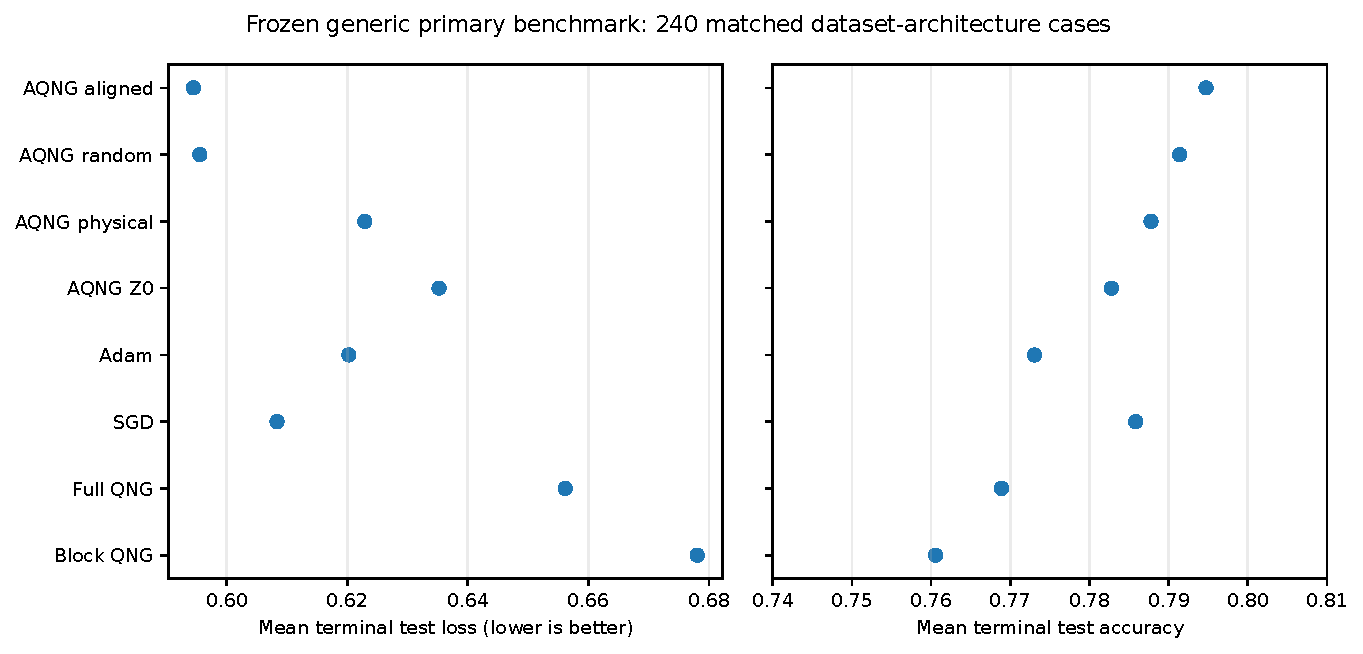
\includegraphics[width=0.96\textwidth]{figures/generated/fig02_generic_primary.pdf}
\caption{Frozen generic primary benchmark pooled over the 240 nonconserving dataset--architecture cases. The primary protocol compares eight methods at matched data partitions and stochastic seeds. Aligned AQNG has the lowest pooled mean terminal test loss (0.5945) and highest pooled mean accuracy (0.7947), but random AQNG and SGD remain close. The pooled means are descriptive summaries; inferential claims use paired tests rather than treating all terminal rows as independent replicates.}
\label{fig:generic_primary}
\end{figure*}

\begin{figure*}[t]
\centering
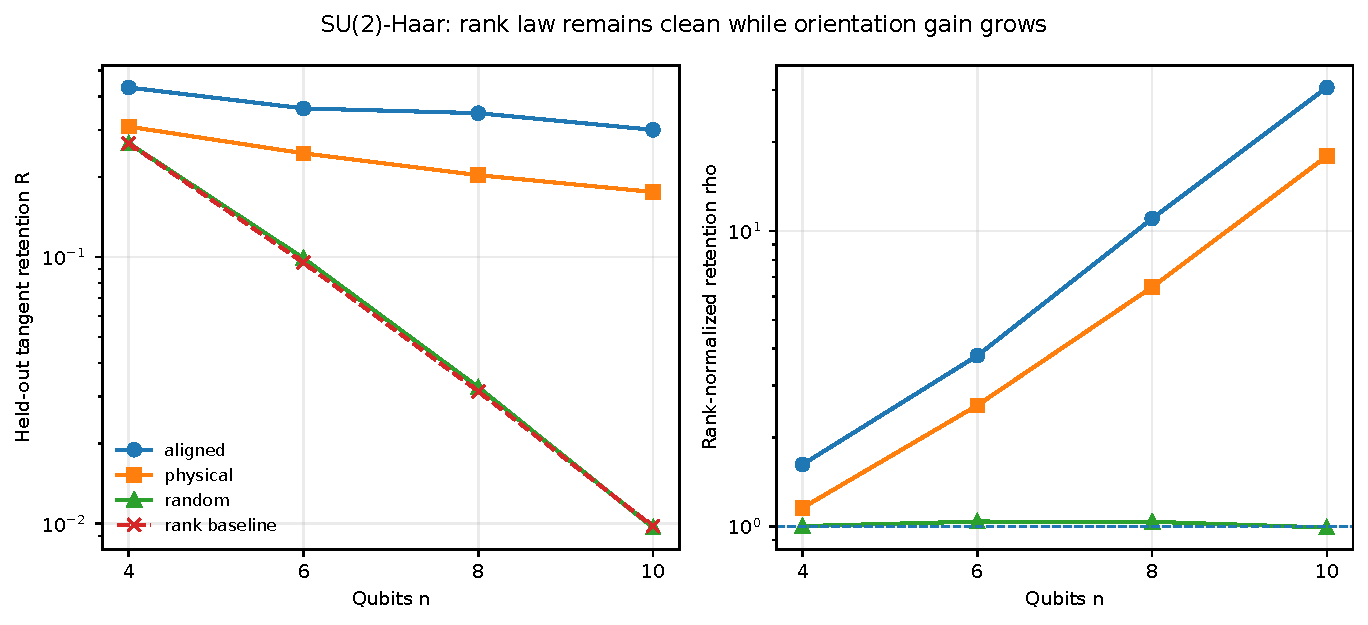
\includegraphics[width=0.96\textwidth]{figures/generated/fig03_scaling_geometry.pdf}
\caption{Qubit scaling of SU(2)-Haar readout geometry at fixed readout order. Left: held-out tangent retention $R$ for cross-fitted aligned, physical, and Haar-random equal-rank readouts, together with the rank-only baseline $r/N$. The baseline falls from $0.267$ at $n=4$ to $9.78\times10^{-3}$ at $n=10$, while the aligned readout still retains about $0.300$ at $n=10$. Right: rank-normalized retention $\rho$. The random control remains near $\rho=1$, whereas the physical and aligned readouts rise to approximately $17.9$ and $30.7$ at $n=10$. The growth is a task-conditioned orientation effect, not a claim that generic physical readouts violate the rank law.}
\label{fig:scaling_geometry}
\end{figure*}

\begin{figure*}[t]
\centering
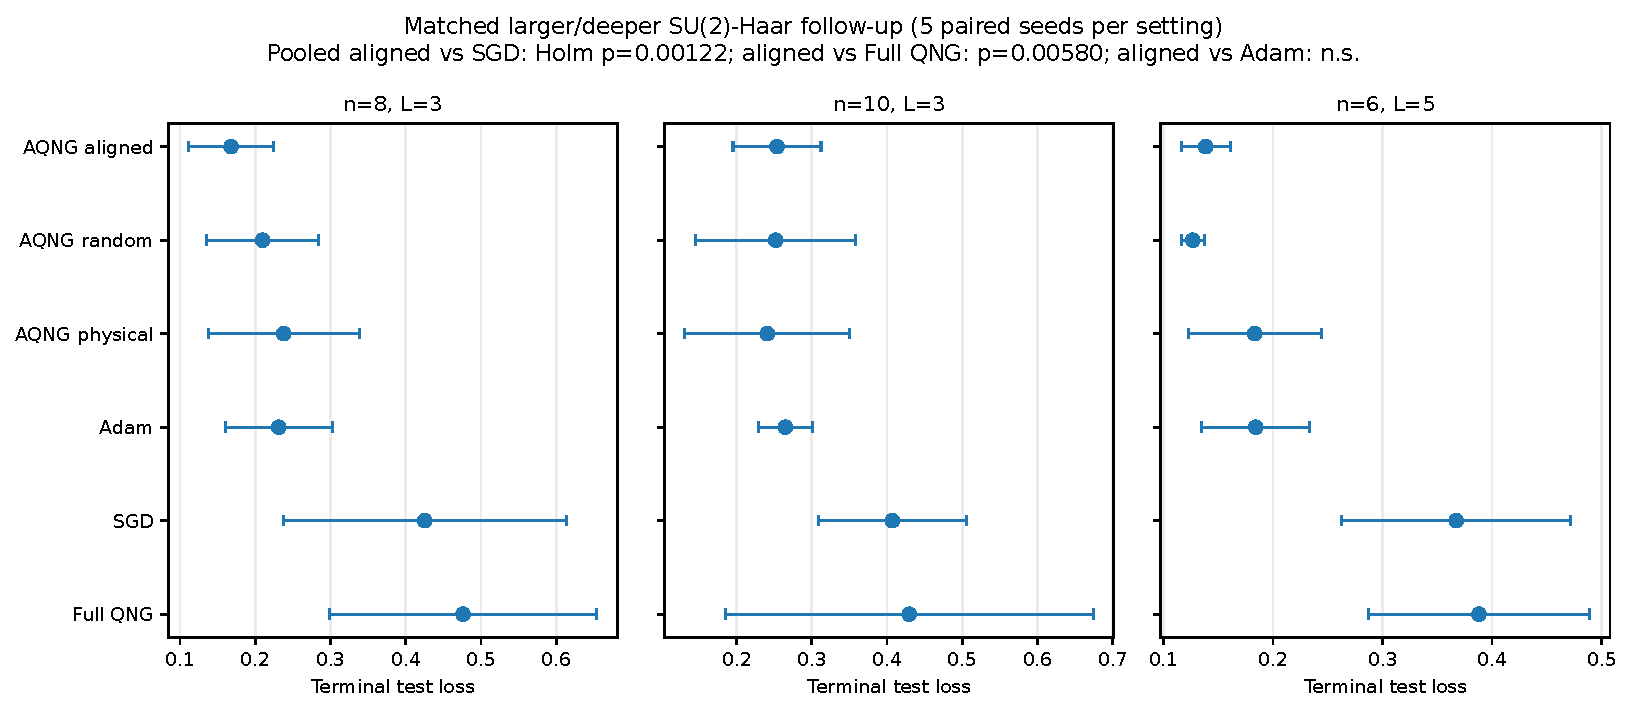
\includegraphics[width=0.98\textwidth]{figures/generated/fig04_large_deep.pdf}
\caption{Matched larger/deeper SU(2)-Haar follow-up. Error bars show the standard deviation across five paired seeds within each setting. Pooled over the 15 matched cells, aligned AQNG beats SGD in 15/15 cases with Holm-adjusted $p=1.22\times10^{-3}$ and full QNG in 14/15 with $p=5.80\times10^{-3}$. The aligned--Adam difference is smaller (10/15 wins) and is not statistically resolved. The follow-up therefore supports a robust advantage over SGD and the tested full-QNG baseline in these regimes, but not universal superiority over Adam.}
\label{fig:large_deep}
\end{figure*}

\begin{figure*}[t]
\centering
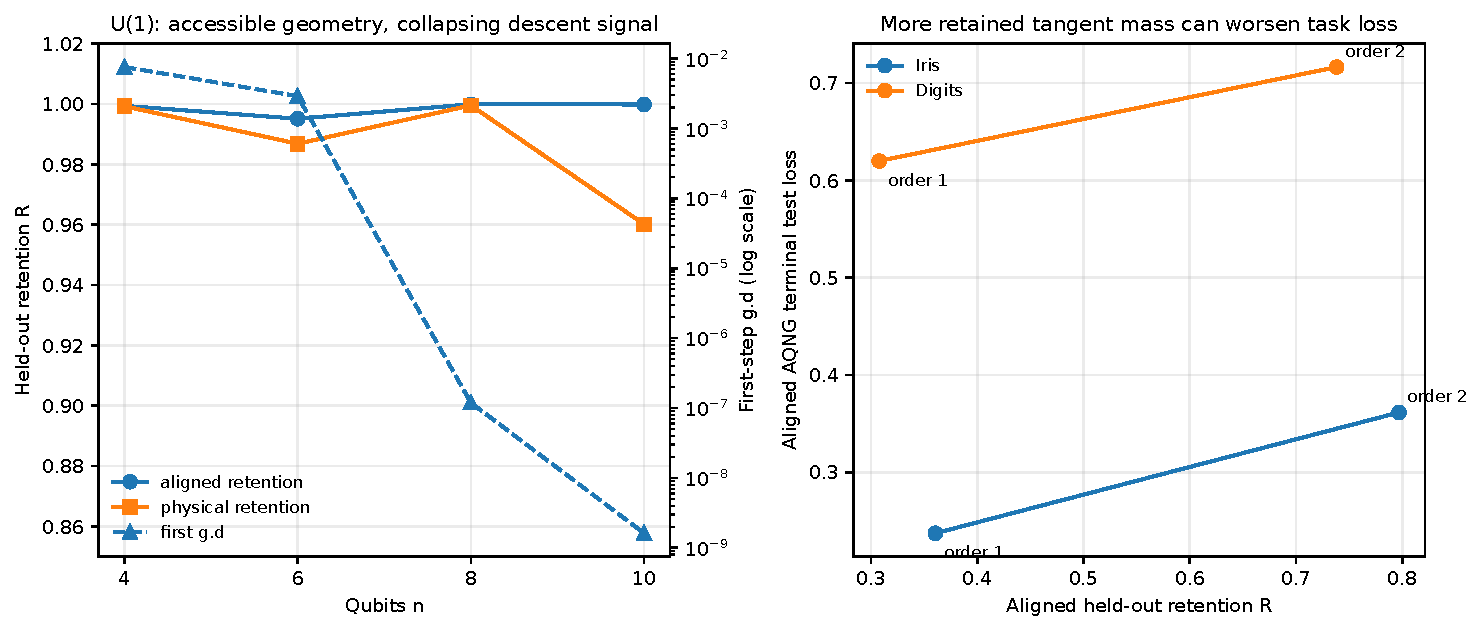
\includegraphics[width=0.98\textwidth]{figures/generated/fig05_accessibility_not_trainability.pdf}
\caption{Accessibility is not trainability. Left: in the half-filled $U(1)$ family, physical and cross-fitted aligned readouts retain nearly all held-out tangent mass over the tested scaling range, while the first-step $g^{\mathsf T}d$ diagnostic collapses by many orders of magnitude and terminal accuracy remains chance-like. Right: for SU(2)-Haar, increasing the readout from order one to order two moves both Iris and Digits toward substantially larger aligned retention but also larger terminal aligned-AQNG loss. Retention is therefore a geometric accessibility diagnostic, not a monotone task-performance objective.}
\label{fig:accessibility_not_trainability}
\end{figure*}

\begin{figure}[t]
\centering
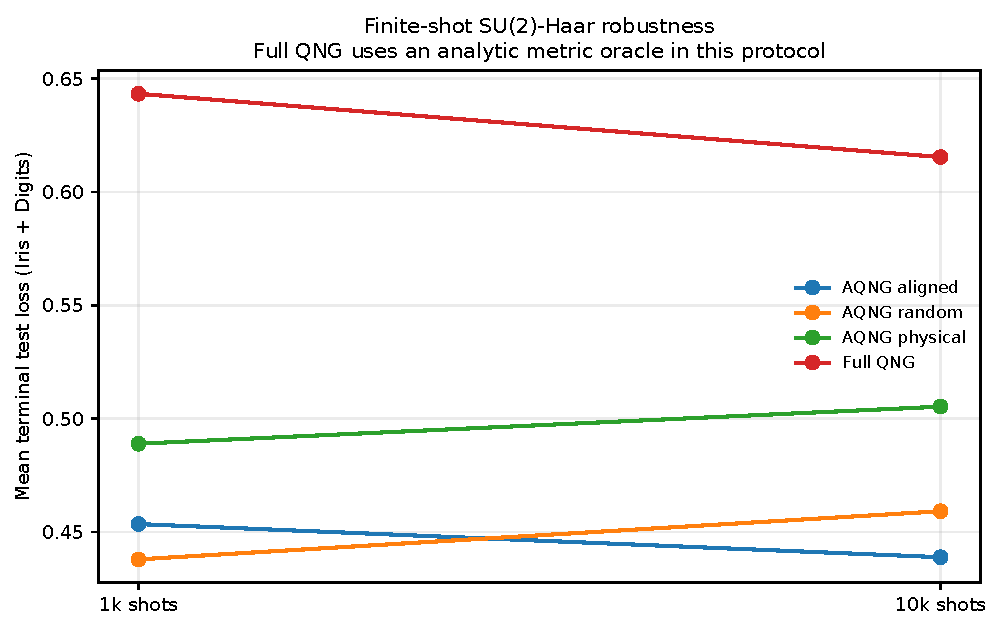
\includegraphics[width=0.98\columnwidth]{figures/generated/fig06_finite_shot.pdf}
\caption{Finite-shot SU(2)-Haar comparison averaged over the Iris and Digits finite-shot cells. AQNG remains competitive at both $10^3$ and $10^4$ shots in the tested protocol, without a monotone terminal-loss improvement as the shot count increases. Full QNG is included as an optimization reference but uses an analytic metric oracle in these finite-shot runs; the figure must therefore not be interpreted as a hardware-fair resource comparison.}
\label{fig:finite_shot}
\end{figure}

\begin{figure*}[t]
\centering
\resizebox{0.94\textwidth}{!}{%
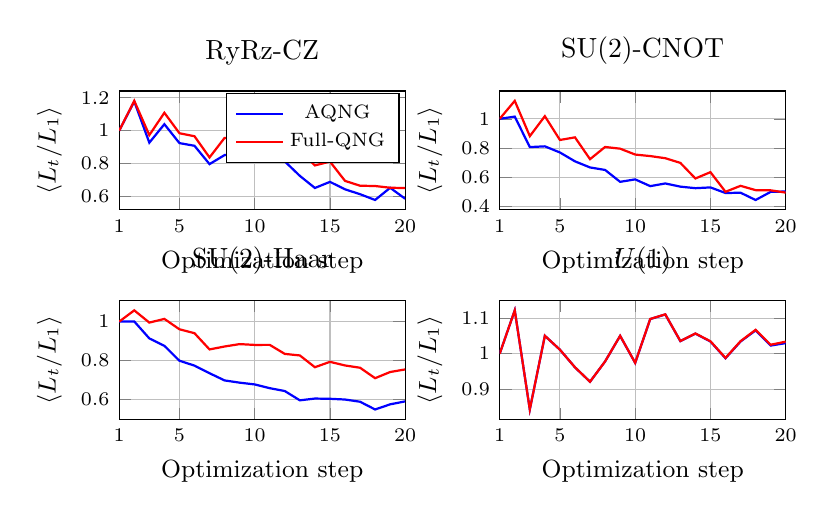
\begin{tikzpicture}
\begin{groupplot}[group style={group size=2 by 2,horizontal sep=1.2cm,vertical sep=1.15cm},
 width=0.43\textwidth,height=0.255\textwidth,
 xmin=1,xmax=20,xtick={1,5,10,15,20},
 xlabel={Optimization step},ylabel={$\langle L_t/L_1\rangle$},
 grid=major,legend style={font=\scriptsize},tick label style={font=\scriptsize},label style={font=\small}]
\nextgroupplot[title={RyRz-CZ}]
\addplot+[thick,mark=none] coordinates {(1,1.000000) (2,1.177099) (3,0.926444) (4,1.038918) (5,0.923778) (6,0.907510) (7,0.795784) (8,0.850791) (9,0.851239) (10,0.826149) (11,0.815254) (12,0.812316) (13,0.724061) (14,0.650395) (15,0.687670) (16,0.642241) (17,0.612473) (18,0.577248) (19,0.651632) (20,0.584484)};
\addlegendentry{AQNG}
\addplot+[thick,mark=none] coordinates {(1,1.000000) (2,1.181105) (3,0.972428) (4,1.108532) (5,0.984041) (6,0.965526) (7,0.836441) (8,0.955582) (9,0.951182) (10,0.937456) (11,0.913793) (12,0.909259) (13,0.876209) (14,0.787698) (15,0.811293) (16,0.693656) (17,0.664103) (18,0.662393) (19,0.651824) (20,0.649922)};
\addlegendentry{Full-QNG}
\nextgroupplot[title={SU(2)-CNOT}]
\addplot+[thick,mark=none] coordinates {(1,1.000000) (2,1.014971) (3,0.806754) (4,0.811720) (5,0.769951) (6,0.709297) (7,0.667441) (8,0.650515) (9,0.569258) (10,0.585922) (11,0.539828) (12,0.558032) (13,0.536379) (14,0.525870) (15,0.531025) (16,0.492775) (17,0.494809) (18,0.445122) (19,0.500506) (20,0.503144)};
\addplot+[thick,mark=none] coordinates {(1,1.000000) (2,1.122558) (3,0.881353) (4,1.017856) (5,0.855254) (6,0.873154) (7,0.724073) (8,0.807452) (9,0.795930) (10,0.755637) (11,0.745210) (12,0.730713) (13,0.698720) (14,0.592075) (15,0.635354) (16,0.501190) (17,0.541919) (18,0.512422) (19,0.511202) (20,0.495583)};
\nextgroupplot[title={SU(2)-Haar}]
\addplot+[thick,mark=none] coordinates {(1,1.000000) (2,1.000728) (3,0.913748) (4,0.875686) (5,0.799100) (6,0.773970) (7,0.734923) (8,0.697935) (9,0.686484) (10,0.677405) (11,0.658116) (12,0.643425) (13,0.595746) (14,0.604843) (15,0.603629) (16,0.599878) (17,0.588473) (18,0.548779) (19,0.575169) (20,0.590425)};
\addplot+[thick,mark=none] coordinates {(1,1.000000) (2,1.057807) (3,0.995003) (4,1.013895) (5,0.960675) (6,0.940512) (7,0.857070) (8,0.872270) (9,0.884472) (10,0.880308) (11,0.880577) (12,0.834163) (13,0.826282) (14,0.765756) (15,0.793460) (16,0.774835) (17,0.763053) (18,0.709480) (19,0.741211) (20,0.754459)};
\nextgroupplot[title={$U(1)$}]
\addplot+[thick,mark=none] coordinates {(1,1.000000) (2,1.122384) (3,0.842460) (4,1.050540) (5,1.011301) (6,0.961469) (7,0.920760) (8,0.977974) (9,1.050267) (10,0.974074) (11,1.097762) (12,1.110807) (13,1.035525) (14,1.056643) (15,1.034405) (16,0.987131) (17,1.034406) (18,1.065777) (19,1.022911) (20,1.029915)};
\addplot+[thick,mark=none] coordinates {(1,1.000000) (2,1.122389) (3,0.842479) (4,1.050567) (5,1.011342) (6,0.961535) (7,0.920835) (8,0.978073) (9,1.050453) (10,0.974273) (11,1.098074) (12,1.111161) (13,1.035938) (14,1.057185) (15,1.035130) (16,0.987960) (17,1.035344) (18,1.067465) (19,1.025308) (20,1.033963)};
\end{groupplot}
\end{tikzpicture}%
}
\caption{Training dynamics from the raw per-step curve logs. For each architecture and optimizer, the minibatch loss is normalized by its first-step value within each run and then averaged over all four datasets and 20 seeds per dataset ($80$ trajectories per curve). The curves therefore show optimizer dynamics rather than terminal test performance. Per-step classification accuracy was not logged in the original run; terminal test accuracy is reported separately in Fig.~\ref{fig:accuracy_all}.}
\label{fig:training_loss}
\end{figure*}

\section{Discussion}
\subsection{From spectral accessibility to an optimizer}
AQNG is the third step in a sequence. The isotropic readout-rank theory showed that state sensitivity can survive while a low-rank readout retains only a small fraction of visible score information \cite{AitHaddouRank}. The spectral theory generalized that result by replacing global isotropy with relative operator alignment $\Tr(TC_Q)$ \cite{AitHaddouSpectral}. AQNG makes this geometry operational by using the accessible tangent structure to precondition learning.

The empirical results support, but do not prove in full generality, the proposition that useful optimization geometry can be smaller than full state-space geometry. SU(2)-Haar is the clearest example: approximately three quarters of QFIM trace is absent from the $\le2$ accessible metric, yet AQNG generalizes better on average across all four benchmarks. Conversely, the $U(1)$ control shows that reproducing the full-QNG direction is not sufficient for task success. This motivates the hierarchy
\begin{equation}
\boxed{\text{state geometry}\;\longrightarrow\;\text{measurement-accessible geometry}\;\longrightarrow\;\text{task-useful optimization geometry}.}
\end{equation}
The first arrow is governed by measurement/readout contraction. The second additionally depends on loss, labels, data encoding, and finite optimization trajectory.

\subsection{Limitations}
The experiments use six-qubit noiseless statevector simulation, small binary datasets, one fixed split per dataset, and 20 optimization steps. They establish a controlled finite-size comparison, not an asymptotic scaling theorem or hardware advantage. AQNG is not guaranteed to outperform full QNG: RyRz-CZ on Digits is a clear counterexample. The timing comparison is also confounded by different metric simulator backends; a matched-backend study should separately count state preparations, circuit evaluations, shots, and classical linear-algebra cost. The present metric uses fixed diagonal readout probes through weight two; general POVMs, rotated bases, adaptive readouts, finite-shot covariance estimation, and noisy channels can alter accessibility. Finally, the $U(1)$ data do not identify the precise source of task failure. Encoding mismatch, conserved-sector expressivity, and readout/label alignment require targeted ablations.

\section{Conclusion}
We introduced the accessible quantum natural gradient, which replaces the full quantum Fisher metric with the metric induced by measurement/readout-accessible tangent geometry. AQNG is motivated by the spectral identity $\mathbb E[I/F_Q]=\Tr(TC_Q)$ and is therefore an algorithmic application of accessible-tangent theory rather than merely a low-cost QFIM approximation.

Across four binary classification datasets, four six-qubit architectures, and 20 paired seeds per cell, AQNG is competitive with full QNG and improves mean accuracy in nine of twelve nonconserving settings. SU(2)-Haar is particularly informative: the accessible metric retains only about one quarter of QFIM trace while AQNG improves mean accuracy on all four tasks, with corrected significant loss gains on Iris and Wine. Digits/SU(2)-CNOT provides a third corrected significant loss gain. The symmetry-constrained $U(1)$ control remains at fixed chance-like accuracy under both optimizers despite strong direction alignment, separating natural-gradient fidelity from task utility.

These results suggest that variational quantum optimization need not reconstruct every locally distinguishable state-space direction. What matters is the geometry that survives the learning interface and is useful to the task. Establishing when this accessible geometry yields provable optimization or sample-complexity advantages is the central open problem raised by AQNG.

\begin{acknowledgments}
The author thanks the open-source scientific Python and quantum-software communities. Computational results and aggregation files are available in the accompanying reproducibility repository \cite{AQNGRepo}.
\end{acknowledgments}

\section*{Data and code availability}
The complete experiment contains 80 dataset--seed jobs and 640 terminal result rows. Aggregate tables, per-seed results, metric diagnostics, and workflow metadata are stored under \texttt{results/paper/paper\_main\_v1/} in Ref.~\cite{AQNGRepo}. The released manifest records the exact workflow configuration and numerical validation tolerance used for reaggregation.

\appendix
\section{Exact AQNG construction used in the experiments}
\label{app:aqng}

This appendix specifies the AQNG instance used for the reported benchmark so that the optimizer can be reconstructed from the experimental record.  We distinguish the mathematical construction from run-time arguments: the former defines the accessible metric, whereas the latter controls its numerical estimation and refresh schedule.

\subsection{Inputs and retained readout family}
For a parameterized circuit $U(\bm\theta)$ on $n$ qubits and an encoded input $x$, AQNG takes (i) the current parameter vector $\bm\theta\in\mathbb R^p$, (ii) a metric minibatch $B_G$, (iii) a retained observable list $\mathcal A=\{O_a\}_{a=1}^{r}$, (iv) a damping coefficient $\lambda$, and (v) a numerical pseudoinverse cutoff $\texttt{rcond}$.  The paper configuration uses the complete diagonal Pauli-$Z$ family through weight two,
\begin{equation}
 \mathcal A_{\le2}=\{Z_i\}_{i=1}^{n}\cup\{Z_iZ_j\}_{1\le i<j\le n}.
\end{equation}
For $n=6$ this gives $r=6+\binom{6}{2}=21$ retained features.  Two smaller spaces are used only as diagnostics: $A_1=\mathrm{span}\{Z_0\}$ and the local space $\mathrm{span}\{Z_i\}_{i=1}^{6}$.  They are not substituted for $\mathcal A_{\le2}$ in the main AQNG training runs.

For each $x\in B_G$, define the retained expectation vector
\begin{equation}
 \bm m(x,\bm\theta)=\big(\langle O_1\rangle,\ldots,\langle O_r\rangle\big)^{\mathsf T},
\end{equation}
its parameter Jacobian $J_x=\partial\bm m/\partial\bm\theta\in\mathbb R^{r\times p}$, and the symmetrized feature covariance
\begin{equation}
 (\Sigma_x)_{ab}=\frac12\langle O_aO_b+O_bO_a\rangle-\langle O_a\rangle\langle O_b\rangle.
 \label{eq:app-cov}
\end{equation}
Because the retained observables are diagonal Pauli-$Z$ strings, they commute in the present implementation.  The covariance-normalized score map is represented by $\Sigma_x^{+1/2}J_x$, with null covariance directions removed by the pseudoinverse.  The per-example accessible Gram matrix is therefore
\begin{equation}
 G_A(x)=J_x^{\mathsf T}\Sigma_x^{+}J_x,
 \label{eq:app-ga-single}
\end{equation}
and the metric used by one refresh is the minibatch average
\begin{equation}
 \widehat G_A(\bm\theta;B_G)=\frac{1}{|B_G|}\sum_{x\in B_G}G_A(x).
 \label{eq:app-ga-batch}
\end{equation}
Equations~\eqref{eq:app-cov}--\eqref{eq:app-ga-batch} are the finite-feature realization of the pullback in Eq.~\eqref{eq:GA}: the Jacobian maps parameter motion into retained readout motion, while $\Sigma_x^{+}$ supplies the covariance/Fisher normalization on that retained motion.

\subsection{Update rule and metric refresh}
Let $B_L$ be the loss minibatch and
\begin{equation}
 \bm g_t=\nabla_{\bm\theta}L(\bm\theta_t;B_L)
\end{equation}
its ordinary parameter gradient.  At a metric-refresh step, AQNG constructs $\widehat G_{A,t}$ from Eq.~\eqref{eq:app-ga-batch}; otherwise it reuses the most recently constructed matrix.  The implemented preconditioned direction is obtained from the damped linear system
\begin{equation}
 (\widehat G_{A,t}+\lambda I)\bm d_t=\bm g_t,
 \qquad
 \bm\theta_{t+1}=\bm\theta_t-\eta\bm d_t.
 \label{eq:app-update}
\end{equation}
A pseudoinverse/SVD cutoff $\texttt{rcond}=10^{-8}$ is used for numerically singular covariance/metric directions.  Damping is applied before the update solve; it regularizes small accessible eigenvalues and prevents null or nearly null retained directions from producing arbitrarily large parameter steps.

The metric is deliberately not rebuilt on every optimization step.  With \texttt{metric\_every}$=2$, the 20-step benchmark performs 10 metric builds.  With \texttt{metric\_batch}$=4$, this corresponds to 40 metric examples per method and seed.  The loss gradient uses \texttt{loss\_batch}$=8$ at each of 20 steps, for 160 loss examples per method and seed.  These logical workloads are matched between AQNG and full QNG; the wall-clock comparison in the main text remains backend-specific.

\subsection{Arguments used in the paper run}
Table~\ref{tab:aqngargs} records the optimizer and experiment arguments preserved by the run manifest and per-seed configuration files.
\begin{table*}
\caption{Arguments of the AQNG benchmark instance.  ``Role'' describes how each argument enters the construction or experimental protocol.}
\label{tab:aqngargs}
\begin{ruledtabular}
\begin{tabular}{lll}
Argument & Paper value & Role\\
\hline
\texttt{n\_qubits} & 6 & Circuit width; gives 21 $Z_{\le2}$ readout features\\
\texttt{n\_layers} & 3 & Variational circuit depth parameter\\
\texttt{steps} & 20 & Number of parameter updates\\
\texttt{learning\_rate} / \texttt{lr} & 0.03 & $\eta$ in Eq.~\eqref{eq:app-update}\\
\texttt{damping} / \texttt{lam} & $10^{-3}$ & Tikhonov damping $\lambda$\\
\texttt{rcond} & $10^{-8}$ & Pseudoinverse/SVD relative cutoff\\
\texttt{loss\_batch} & 8 & Examples used for each loss gradient\\
\texttt{metric\_batch} & 4 & Examples averaged in each metric refresh\\
\texttt{metric\_every} & 2 & Rebuild metric every second optimization step\\
\texttt{readout} & $Z_{\le2}$ & All $Z_i$ and $Z_iZ_j$ retained observables\\
\texttt{n\_samples} & 80 & Dataset subset size used in each benchmark\\
\texttt{subset\_seed} & 1729 & Fixed seed selecting the dataset subset\\
\texttt{split\_seed} & 314159 & Fixed train/test split seed\\
\texttt{seed} & 0--19 & Initialization, minibatch schedule, and fixed Haar instance\\
\end{tabular}
\end{ruledtabular}
\end{table*}
The stochastic seed does \emph{not} change the train/test split.  It controls parameter initialization, minibatch scheduling, and, for \texttt{su2\_haar}, the fixed Haar entangling instance.  Thus the 20 repetitions probe training/circuit stochasticity on one fixed split per dataset.

\subsection{Reference algorithm}
The complete AQNG iteration can be summarized as follows:
\begin{enumerate}
 \item Fix the retained observable family $\mathcal A_{\le2}$ and initialize $\bm\theta_0$.
 \item At step $t$, draw the paired loss minibatch $B_L$ and evaluate $\bm g_t=\nabla L(\bm\theta_t;B_L)$.
 \item If $t$ is a refresh step, draw $B_G$; for every $x\in B_G$, evaluate $\bm m(x,\bm\theta_t)$, $J_x$, and $\Sigma_x$, then form $G_A(x)=J_x^{\mathsf T}\Sigma_x^+J_x$ and average the four matrices.  Otherwise reuse the preceding $\widehat G_A$.
 \item Solve $(\widehat G_A+\lambda I)\bm d_t=\bm g_t$ using the stated numerical cutoff.
 \item Update $\bm\theta_{t+1}=\bm\theta_t-\eta\bm d_t$.
\end{enumerate}
Full QNG follows the same loss minibatches, metric minibatch size, refresh cadence, damping, and learning rate, but replaces $\widehat G_A$ by the full pure-state QFIM.  This pairing is why the initial gradient is identical up to floating-point precision and why differences can be attributed to the preconditioning geometry rather than to a different stochastic workload.

\subsection{Diagnostics and consistency checks}
At the initial paired point the implementation additionally constructs $G_{A_1}$, $G_{\rm local}$, $G_{\le2}$, and $G_Q$.  It records their ranks and traces, the ratios $\Tr(G_{\mathcal A})/\Tr(G_Q)$, and the cosine between each preconditioned direction and the full-QNG direction.  It also checks the nested Loewner ordering
\begin{equation}
 G_{A_1}\preceq G_{\rm local}\preceq G_{\le2}\preceq G_Q.
\end{equation}
The production run used a scale-aware numerical validation tolerance of order $10^{-5}$ in the pre-run smoke gate.  The largest observed nesting residual was $8.706\times10^{-6}$ in Wine/$U(1)$; no training datum or terminal statistic was modified during reaggregation.

\subsection{Scope of the implementation description}
The equations above specify the accessible metric and all numerical arguments recorded for the reported run.  They should not be read as requiring diagonal Pauli readout in general.  For a different measurement/readout interface, $\bm m$, $J$, and $\Sigma$ are replaced by the corresponding retained score coordinates; the abstract construction remains the pullback of the accessible tangent map.  Likewise, \texttt{metric\_batch}, \texttt{metric\_every}, $\lambda$, and \texttt{rcond} are numerical hyperparameters rather than defining properties of AQNG itself.


\bibliography{references}
\end{document}
